\documentclass[12pt]{article}
\usepackage{amsmath}
%\usepackage{fullpage}
\usepackage[top=1in, bottom=1in, left=0.8in, right=1in]{geometry}
\usepackage{multicol}
\usepackage{wrapfig}
\usepackage{graphicx}
\usepackage{float}
\usepackage{listings}
\usepackage{enumerate}
\lstset{language=Java,
	basicstyle={\small\ttfamily},
	columns=flexible,
	belowskip=0mm}

\setlength{\columnsep}{0.1pc}

\title{ME573 Homework Set \# 8}
\author{Alexander Swenson -- \texttt{aaswenson@wisc.edu}}
\date{\today}
\begin{document}
	
	\maketitle
	
	\vspace{-0.3in}
	\noindent
	\rule{\linewidth}{0.4pt}
	
	\noindent
	
	%%%%%%%%%%%%%%%%%%%%%%%%%%%%%%%%%%%%%%%%%%%%%%%%%%%%%%%%%%%%%%%%%%%%%%%%%%%%%%%%
	% Problems 1
	
	\section{Introduction}
	
	\noindent This coding assignment involved solving a Second-Order PDE with iterative methods. The three iterative methods tested were: Jacbobi iteration, Gauss-Seidel, and Successive Over-Relaxation.
	
	%%%%%%%%%%%%%%%%%%%%%%%%%%%%%%%%%%%%%%%%%%%%%%%%%%%%%%%%%%%%%%%%%%%%%%%%%%%%%%%%
	
	\section{Problem 1}
	
	\noindent Each method was tested on a unit square. The L1 error of each method was calculated with increasing number of iterations from 2-800. The impact of number of iterations on the L1 error is shown in the following three plots. Each plot shows the L1 error as a function of N iterations at different dx values. All three methods were tested using MATLAB (2016a).
	
	\begin{figure}[H]
		\centering
		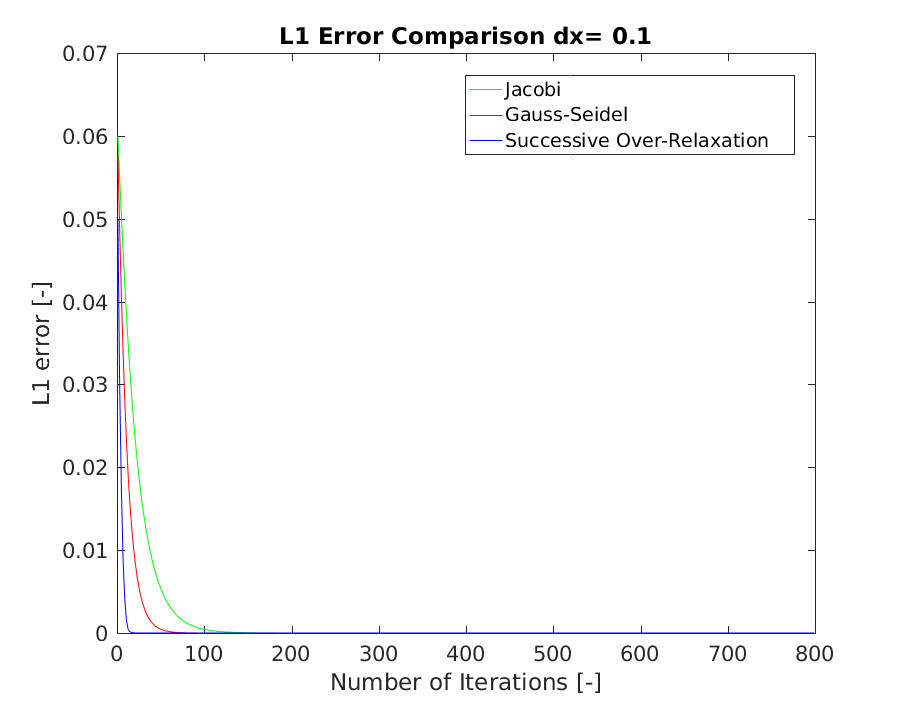
\includegraphics[height=3.75in]{p1_01.png}
		\label{fig:problem2_plot}
	\end{figure}
	
	\begin{figure}[H]
		\centering
		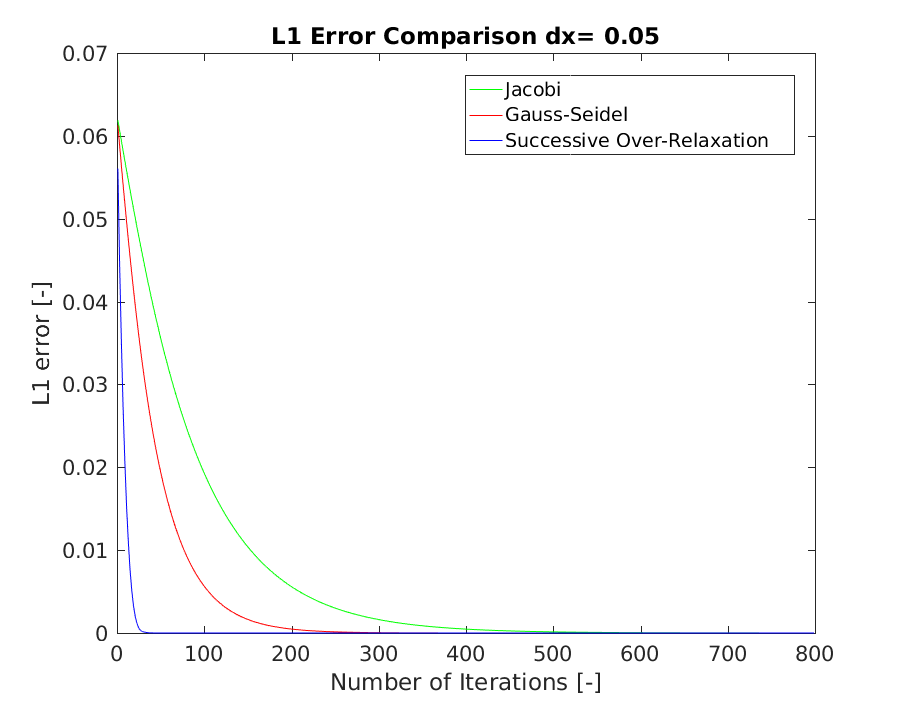
\includegraphics[height=3.75in]{p1_005.png}
		\label{fig:problem2_plot}
	\end{figure}
		
	\begin{figure}[H]
		\centering
		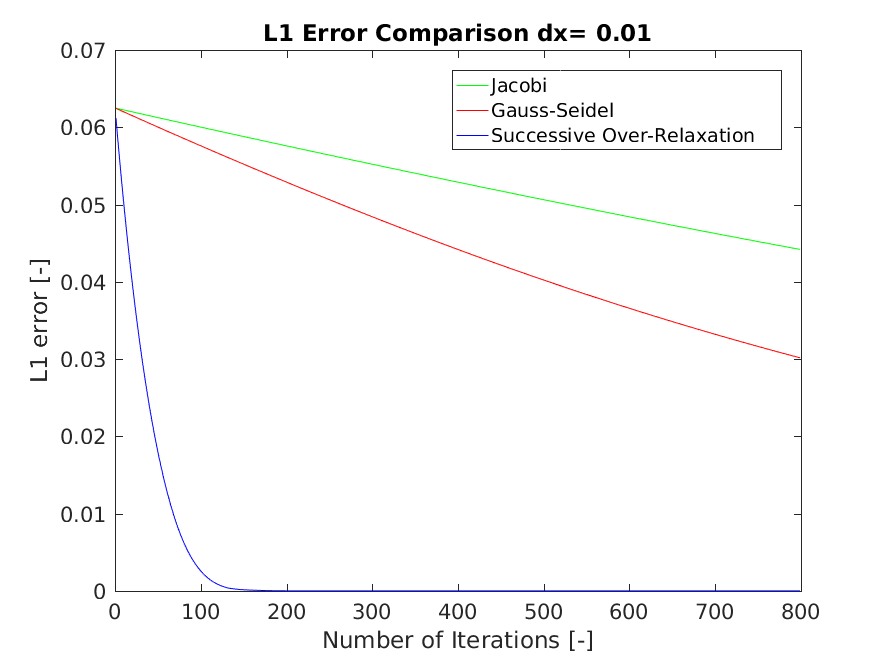
\includegraphics[height=3.75in]{p1_001.png}
		\label{fig:problem2_plot}
	\end{figure}
	
	
	%%%%%%%%%%%%%%%%%%%%%%%%%%%%%%%%%%%%%%%%%%%%%%%%%%%%%%%%%%%%%%%%%%%%%%%%%%%%%%%%
	
		
	\section{Problem 2}
	
	The following iteration decomposition was considered and shown to hold for SOR.
	
	\begin{equation}
		\textbf{Mu}^{k+1} = \textbf{Bu}^k + \textbf{b}
	\end{equation}
	
	\begin{equation}
	\textbf{Au}=\textbf{b}
	\end{equation}
	
	\begin{equation}
	\textbf{Au}=\textbf{b}
	\end{equation}
	
	\begin{equation}
	\textbf{A}=\textbf{D-L-U}
	\end{equation}
	
	\noindent Show the following holds.
	
	\begin{equation}
	\textbf{M}=\frac{1}{\omega}(\textbf{D}-\omega\textbf{L})
	\end{equation}
	
	\begin{equation}
	\textbf{N} = \frac{1}{\omega}[(1-\omega)\textbf{D} + \omega\textbf{U}]
	\end{equation}

\noindent First, start with some substitution (5 \& 6 into 1)

\begin{equation}
\frac{1}{\omega}(\textbf{D}-\omega\textbf{L})\textbf{u}^{k+1} = \frac{1}{\omega}[(1-\omega)\textbf{D} + \omega\textbf{U}]\textbf{u}^k + \textbf{b}
\end{equation}

\begin{equation}
(\textbf{D}-\omega\textbf{L})\textbf{u}^{k+1} = [(1-\omega)\textbf{D} + \omega\textbf{U}]\textbf{u}^k + \omega \textbf{b}
\end{equation}

\begin{equation}
(\textbf{D}-\omega\textbf{L})\textbf{u}^{k+1} = \textbf{Du}^k - \omega\textbf{Du}^k + \omega\textbf{Uu}^k + \omega \textbf{Du}^k - \omega\textbf{Lu}^k - \omega \textbf{Uu}^k
\end{equation}

\begin{equation}
(\textbf{D}-\omega\textbf{L})\textbf{u}^{k+1} = \textbf{Du}^k - 2\omega \textbf{Uu}^k - \omega \textbf{Lu}^k
\end{equation}

\begin{equation}
\textbf{u}^{k+1} = \frac{\textbf{Du}^k - 2\omega \textbf{Uu}^k - \omega \textbf{Lu}^k}{(\textbf{D}-\omega\textbf{L})}
\end{equation}




%%%%%%%%%%%%%%%%%%%%%%%%%%%%%%%%%%%%%%%%%%%%%%%%%%%%%%%%%%%%%%%%%%%%%%%%%%%%%%%%

		
	
	
	
	
\end{document}
